\chapter{Simulated annealing and methods for exploring Gibbs distributions}
\chaptermark{Simulated annealing}

Let $\mathcal{C}$ and $\mathcal{X}$ be a hypothesis class and an instance space, respectively. Let
also $R$ be a cost function. We are interested in the distribution $p(\cdot \mid X)$,
for a given $X \in \mathcal{X}$. In practice, however, the complexity of $R$ makes often
$p(\cdot \mid X)$ \emph{analytically intractable}: there is no known analytical technique to
use $p(\cdot \mid X)$ to make predictions. In other cases, the size of $\mathcal{C}$ is so large that
computing the normalization constant of this distribution \emph{computationally
intractable}: there is no known efficient algorithm for computing the value
of $p(c \mid X)$, for every $c \in \mathcal{C}$.

This chapter explores methods for computationally handling and eventually
extracting useful models from $p(\cdot \mid X)$, all of them based in sampling.
These methods were originally proposed for optimization, but we use them
here to produce samples of $p(\cdot \mid X)$ that are concentrated around a local
minimum of $R(\cdot, X)$. Moreover, in the case of a particular technique called \emph{simulated annealing}, it has
been formally demonstrated that when its hyper-parameters are adjusted
properly, the samples concentrate around a global minimum of $R(\cdot, X)$.

\section{Chapter overview}

We have seen how the Gibbs distribution concentrates on the global minima
of $R(\cdot, X)$ as the temperature converges to zero. This is advantageous over
ERM methods, as it gives us more candidate models aside from the empirical
risk minimizer that not only have a lower cost but can also generalize
better. Unfortunately, in practice, this Gibbs distribution is intractable,
mainly because of its normalization constant.

One way to go around this intractability is via sampling. There are
methods for sampling intractable distributions that are effective and popular.
We show how to use sampling to explore the Gibbs distribution and
choose models from it.

A popular method to sample intractable distributions is by MCMC
sampling, which we study in Section~\ref{sec:mcmc}. However, MCMC is impractical
for sampling Gibbs distributions. We will see in Section~\ref{sec:mcmc_traversal} that the lower
the temperature of the Gibbs distribution, the more time MCMC requires
to produce a useful sample, as consecutive samples tend to accumulate in
the neighborhood of a local minima of the cost function. We will also see
that when the temperature is high MCMC works well. Unfortunately, in
this case the Gibbs distribution does not substantially discriminate between
good and bad models.

We study simulated annealing (SA) in Section~\ref{sec:simulated_annealing} and see how it overcomes
this limitation of MCMC \emph{by decreasing the temperature during the
MCMC sampling}. SA starts by setting the temperature to a very large
value, so that the Gibbs distribution is almost uniform and MCMC efficiently produces samples. After some samples, SA alternates between decreasing
the current temperature and drawing more samples. We will see,
albeit informally, that the alternation between sampling and temperature
decreasing avoids that SA gets stuck in the neighborhood of a bad local
minimum. It can be formally proven that when the temperature decreasing
schedule is done properly, SA converges to the cost function's global
minimum.

Simulated annealing offers two advantages over the standard empirical
risk minimization (ERM). First, it can converge to a global minimum, or
at least to a local minimum of good quality. Second, the sampling nature
of SA gives not only one but several models to choose from. In contrast,
ERM tends to produce only one model that is just local minima of the
cost function. As seen in the random array problem from Section 1.4, this
model may not generalize well.

In the case of clustering, the stochastic nature of SA makes it superior
to ERM methods like K-means, as we will study in Chapter 3. Moreover,
we will see that in several instances, SA can be improved to a more exact
and simpler method, called \emph{deterministic annealing} (DA).

\section{Sampling as a way to extract models from Gibbs distributions}
\label{sec:sampling}

In many interesting cases in practice, $p(\cdot \mid X)$ is intractable. However, there
are effective methods for sampling intractable distributions. Sampling gives
us a way to explore and to choose a model from $p(\cdot \mid X)$, when $\mathcal{C}$ is a vector
space, or at least a space that admits a notion of an average: draw a sample from $p(\cdot \mid X)$ and then propose the average of that sample as a model.
Figure~\ref{fig:two_observations_sa} illustrates two observations from the random array problem
from Section~\ref{sec:random_array}. Here, the array has length 100. The upper graphic in Figure~\ref{fig:means_pas_two_arrays} illustrates the mean of the two Gibbs distributions induced by
$R(\cdot, X')$ and $R(\cdot, X'')$ as a function of the temperature. Observe that in
this case, the mean would then be the model that we would choose, if we
could only access $p(\cdot \mid X')$ or $p(\cdot \mid X'')$ via sampling. The lower graphic in Figure~\ref{fig:means_pas_two_arrays}
illustrates the kernel posterior agreement between the two observations as
a function of the temperature.

\begin{figure}[hbtp]
\centering
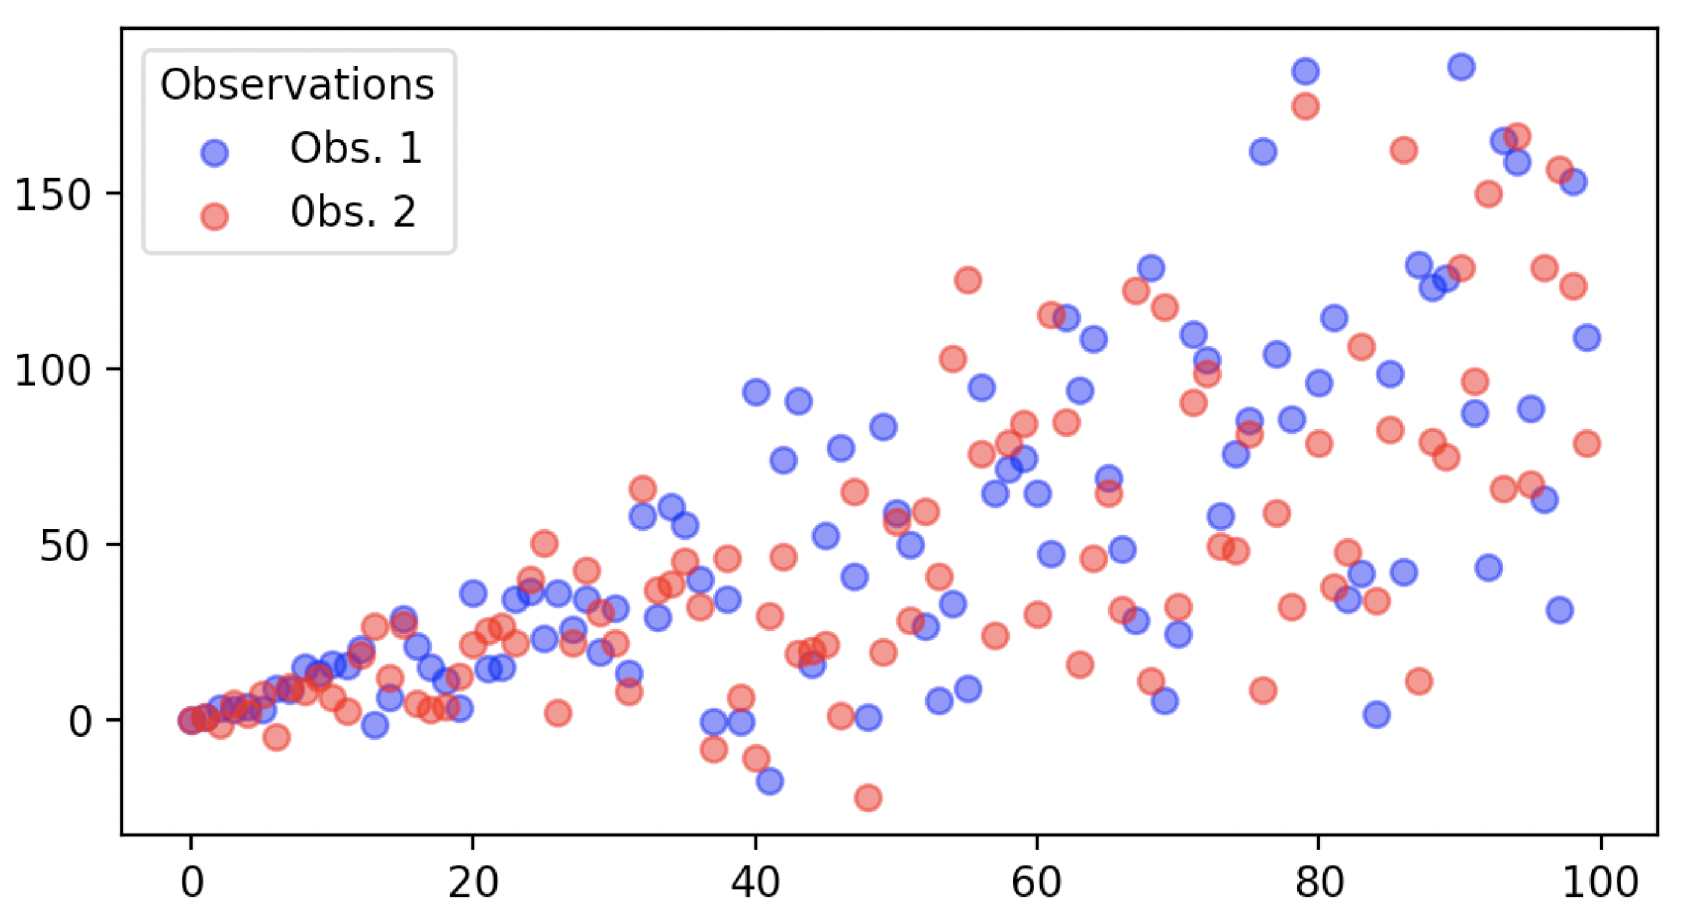
\includegraphics[width=\textwidth]{\dir/two_observations}
\caption{}
\label{fig:two_observations_sa}
\end{figure}

\begin{figure}[hbtp]
\centering
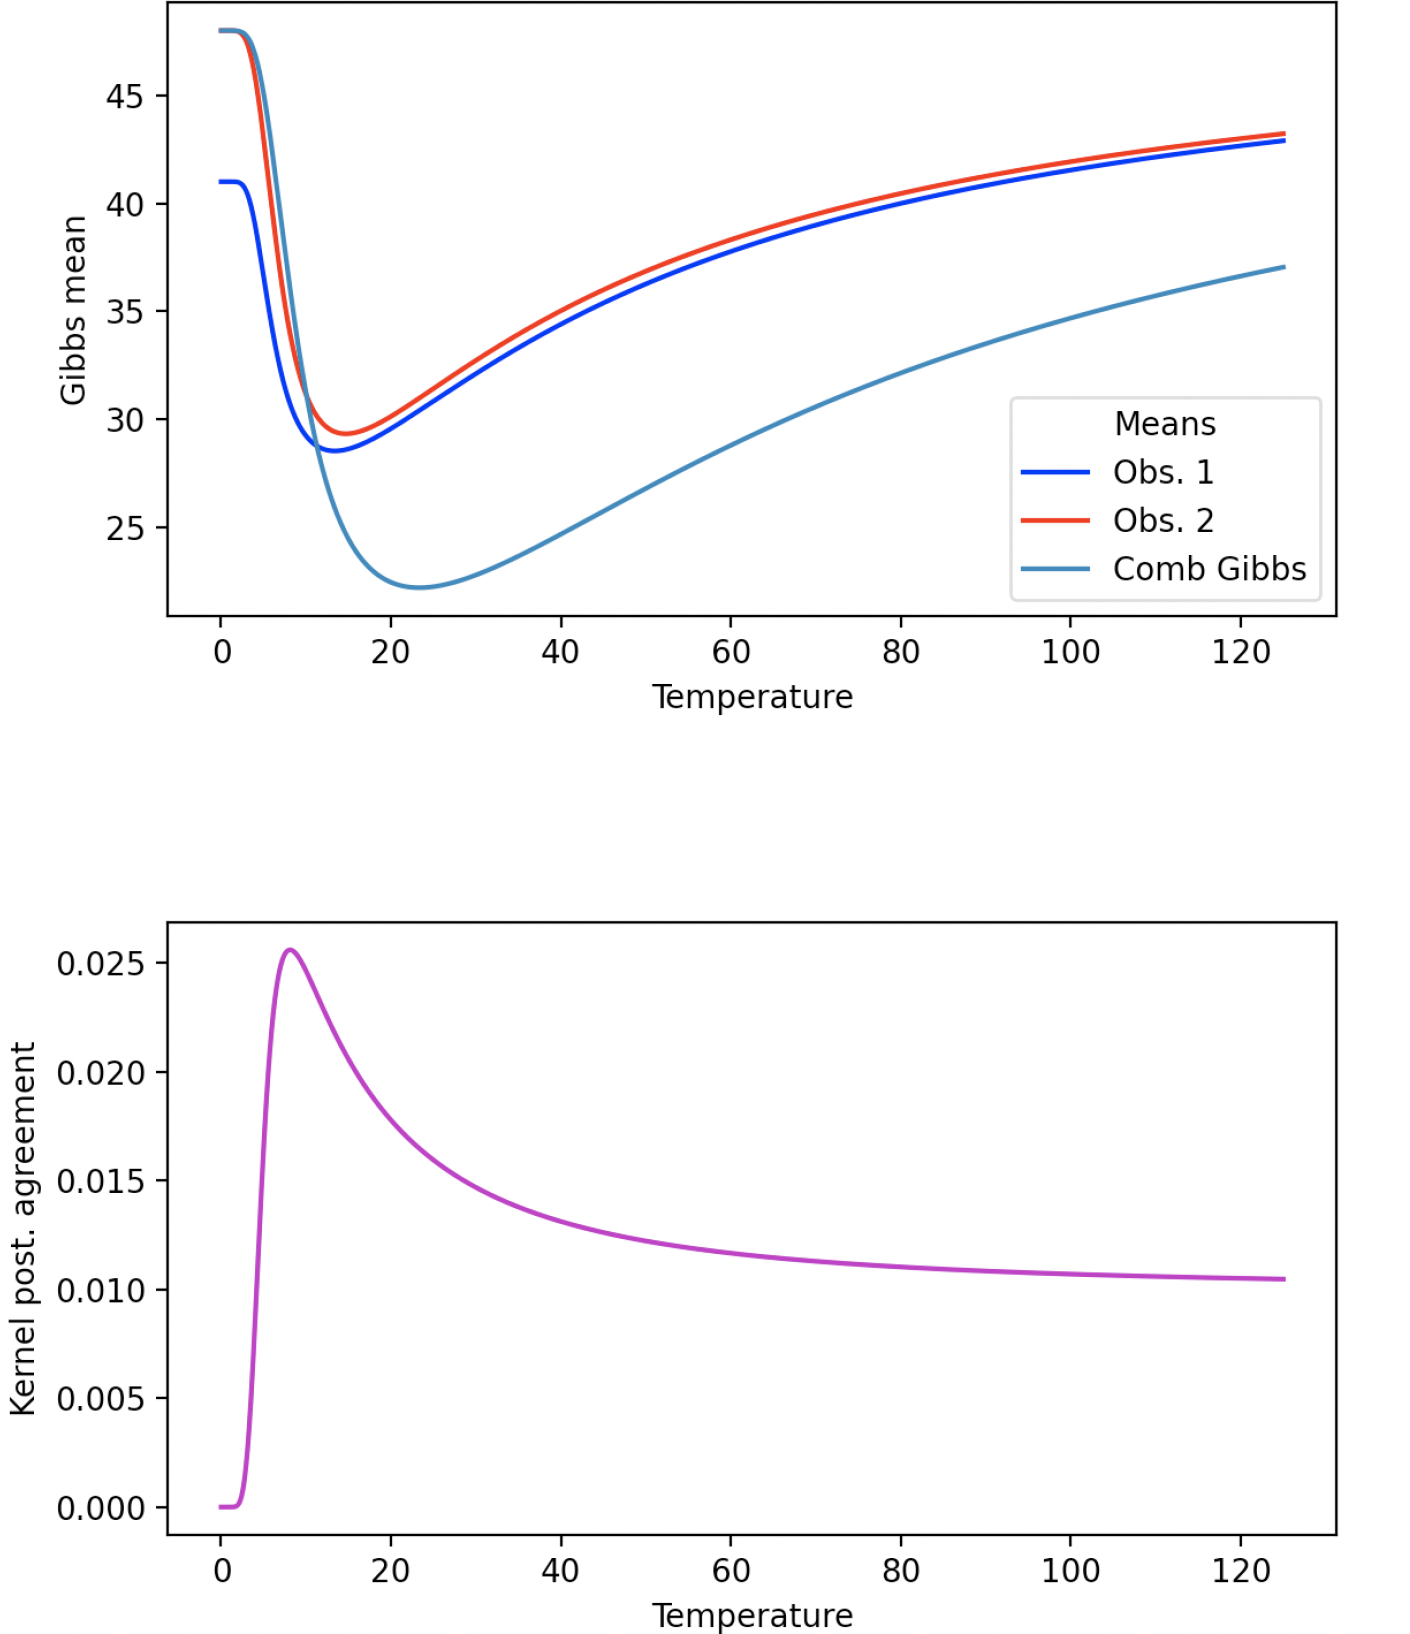
\includegraphics[width=\textwidth]{\dir/means_pas_two_arrays}
\caption{}
\label{fig:means_pas_two_arrays}
\end{figure}

As $T \to \infty$, the mean of the two Gibbs distributions lie near to 50. This
is because at a sufficiently high temperature, the Gibbs distributions look
like uniform distributions. As the temperatures start decreasing, the distributions
concentrate more and more on the array entries with the lowest
values. Such values are in the first half of the array. This is why the means
decrease as the temperature decreases from 120 to 20 for the two Gibbs
distributions. However, the means start increasing when the temperature
gets below 20. This is because the Gibbs distributions start concentrating
on the arrays' minima. In particular, when the temperature approaches
zero, the distributions concentrate almost entirely on the minima of the
corresponding arrays. The combined Gibbs distribution has a similar behavior.

When searching for a good model in the Gibbs distribution, it is important
to choose an adequate value of the temperature. We argue that
such a value can be computed by maximizing the kernel posterior agreement
between two given observations. Observe in the lower graphic of
Figure~\ref{fig:means_pas_two_arrays} that the temperature at which the kernel posterior agreement is
maximum is very close to the temperature at which the means of the two Gibbs distributions are minimized.


\section{MCMC sampling}
\label{sec:mcmc}

MCMC sampling is one of the most popular methods for sampling from
intractable distributions, especially when the source of intractability is the
normalization constant. We give here a basic recap of MCMC. For a more
thorough overview, please refer to Bishop's ``Pattern recognition and machine
learning'' or Murphy's ``Machine learning: a probabilistic perspective''.

\subsection{Markov chain Monte Carlo}

Given a distribution $p$, MCMC sampling is usually done by defining a
parameterized family of conditional \emph{transition distributions} $\pi(\cdot \mid c)$, for an
arbitrary $c \in \mathcal{C}$. This distribution gives rise to a graph $G$ whose vertices
are $\mathcal{C}$ and where there is an edge between any two $c, c' \in \mathcal{C}$ iff $\pi(c' \mid c) > 0$.
MCMC sampling then proceeds to produce samples iteratively as follows.
First, pick an arbitrary $C_0 \in \mathcal{C}$. Then for $t = 1, 2, \ldots$, sample $C_t$ from $\pi\left(\cdot \mid C_{t-1}\right)$. The samples eventually look like samples from $p$ if the conditions
below are met.

\begin{theorem}
Let $p$ be a distribution over $\mathcal{C}$ and let $\{\pi(\cdot \mid c)\}_{c \in \mathcal{C}}$ be a parameterized
family of conditional distributions on $\mathcal{C}$ meeting the following
requirements.

\begin{itemize}
\item $G_\pi$ is connected.
\item There is an edge from a vertex to itself in $G_\pi$.
\item $\pi(c' \mid c)p(c) = \pi(c \mid c')p(c')$, for any two $c, c' \in \mathcal{C}$.
\end{itemize}

Let $C_0, C_1, \ldots$ be a sequence of random variables such that, for $1 \leq t$,
$C_t$'s distribution is given by $\pi(\cdot \mid C_{t-1})$. Then, for $c \in \mathcal{C}$,
%
\begin{equation}
\lim_{t \to \infty} \prob\left(C_t = c\right) = p(c).
\end{equation}
%
\label{thm:convergence_markov}
\end{theorem}

The proof is found in standard probability textbooks and is studied in
the course \emph{probabilistic artificial intelligence}.

\subsection{The Metropolis-Hastings trick}

MCMC gives a simpler recipe to sample an intractable distribution $p$: just
come up with a transition distribution fulfilling the three requirements
from Theorem~\ref{thm:convergence_markov}. The hardest requirement is the last one, called detailed
balance, as it demands a good understanding of $p$ in order to fulfil that
equation. Fortunately, there is a convenient trick proposed by Metropolis
and Hastings that easily yields such a transition distribution.

The trick works for distributions where the intractability comes from
the normalization constant, which is often the case in Bayesian methods
and in our Gibbs distributions. So let us assume that $p(c) \propto f(c)$, where
$f(c)$ is tractable. The trick consists of two steps:

\begin{enumerate}
\item Define a parameterized family of conditional proposal distributions
$\{q(\cdot \mid c) \mid c \in \mathcal{C}\}$ such that $G_q$ is connected and every vertex in $G_q$
has an edge to itself.
\item Define, for $c, c' \in \mathcal{C}$, the \emph{accepting probability}
%
\begin{equation}
A(c', c) := \min\left\{1, \frac{q(c \mid c')p(c')}{q(c' \mid c)p(c)}\right\} = \min\left\{1, \frac{q(c \mid c')f(c')}{q(c' \mid c)f(c)}\right\}.
\end{equation}
%
\end{enumerate}

\begin{exercise}
Let $c \in \mathcal{C}$ and
%
\begin{equation}
\pi(c' \mid c) := \begin{cases}
q(c' \mid c)A(c', c) & \text{if $c \neq c'$ and}\\
1 - \sum_{c' \neq c}q(c' \mid c)A(c', c) & \text{otherwise}.
\end{cases}
\end{equation}
%
Show that $\pi(\cdot \mid c)$ fulfils the requirements from Theorem 1.
\end{exercise}

\begin{exercise}
In our context, we usually choose proposal distributions $q(\cdot \mid \cdot)$
that are symmetric. That is, $q(c' \mid c) = q(c \mid c')$ for $c, c' \in \mathcal{C}$. Show that,
in this case, the Metropolis-Hastings transition distribution $\pi(\cdot \mid c)$ for a
Gibbs distribution $p(c \mid X) \propto \exp\left(-\frac{1}{T}R(c, X)\right)$ simplifies to the following:

\begin{itemize}
\item If $c \neq c'$ and $R(c', X) > R(c, X)$, then $\pi(c' \mid c) = q(c' \mid c)\rho(c, c')$, where $\rho(c, c') = \exp\left(\frac{1}{T}\left(R(c, X) - R(c', X)\right)\right)$.
\item Otherwise, if $c \neq c'$ and $R(c', X) \leq R(c, X)$, then $\pi(c' \mid c) = q(c' \mid c)$.
\item Otherwise,
%
\begin{equation}
\pi(c' \mid c) = 1 - \sum_{c' : R(c', X) \leq R(c, X)}q(c' \mid c) - \sum_{c': R(c', X) > R(c, X)}q(c' \mid c)\rho(c, c').
\end{equation}
%
\end{itemize}
\end{exercise}

For $c \in \mathcal{C}$, we can then draw a sample $C$ from $\pi(\cdot \mid c)$ in two easy steps:

\begin{enumerate}
\item Draw a sample $\tilde{C}$ from $q(\cdot \mid c)$.
\item If $R(\tilde{C}, X) > R(c, X)$, then draw a sample $b$ from a Bernoulli distribution with mean $\exp\left(\frac{1}{T}\left(R(c) - R(\tilde{C})\right)\right)$. If $b = 1$, then $C:= \tilde{C}$. Otherwise, $C := c$.
\end{enumerate}

\subsection{MCMC sampling of Gibbs distributions}

We now summarize all our insights so far. Assume given a Gibbs distribution $p(c \mid X) \propto \exp\left(-\frac{1}{T}R(c, X)\right)$. The normalization constant
$\sum_{c} \exp\left(-\frac{1}{T}R(c, X)\right)$,
also called \emph{the partition function}, is intractable in most of the interesting
cases. We are interested in models that have a high probability mass according
to this distribution, as we believe that some of them generalize
very well. To retrieve these models without dealing with the intractability
of $p(c \mid X)$, we do the following.

\begin{enumerate}
\item Define a symmetric proposal distribution $q(\cdot \mid c)$ such that $G_1$ is
connected and every vertex in $G_q$ has an edge to itself.
\item Let $C_0$ be an arbitrary element in $C$.
\item For $t = 1, 2, \ldots$, draw a sample $C_t$ from $\pi(\cdot \mid C_{t-1})$as explained
above.
\end{enumerate}

By Theorem~\ref{thm:convergence_markov}, the samples produced by this algorithm eventually become
samples of $p(\cdot \mid X)$.

It is important to emphasize that MCMC and the Metropolis-Hastings
trick are not restricted only to Gibbs distributions. These sampling techniques
have existed for decades and are still very popular today for dealing
with intractable distributions.

\section{MCMC sampling as a randomized traversal algorithm}
\label{sec:mcmc_traversal}

Before we continue, we give a toy example that gives us some intuitions
of how MCMC sampling works for Gibbs distributions. We argue that
MCMC sampling of $p(\cdot \mid X)$ can be understood with a parable of a treasure
hunter that explores the hypothesis class $\mathcal{C}$ in a random way, searching
for local minima of $R(\cdot, X)$. The sequence of locations visited by the hunter
correspond to the sequence of samples drawn via MCMC. When the temperature
is low, this hunter lingers in local minima of $R(\cdot, X)$ that are close
to the hunter's starting position. When the temperature is high, the hunter
roams over $\mathcal{C}$, showing little preference over the different local minima of $R(\cdot, X)$.

In the next section, we explain why this is problematic in practice: for
the Gibbs distribution to be useful for us, it must have a sufficiently low
temperature so that its probability mass is concentrated on valuable local
minima of $R(\cdot, X)$. However, such a low temperature prevents MCMC to
leave bad local minima and makes the success of MCMC very sensitive to
the choice of the intial sample, making MCMC impractical for our analyzing
Gibbs distributions. Afterwards, we show how simulated annealing solves
this issue.

\subsection{Illustrative example}

Let $C = \{0, 1, \ldots, 24\}$ and consider the cost function $R(\cdot, X)$ in Figure~\ref{fig:chainsaw_sa},
where $X$ is some arbitrary observation. The horizontal axis describes the
models in $\mathcal{C}$. The vertical axis denotes $R(c, X)$, for some $c \in \mathcal{C}$. Notice
that the minimizer of $R(\cdot, X)$ is $c^* = 19$.

\begin{figure}
\centering
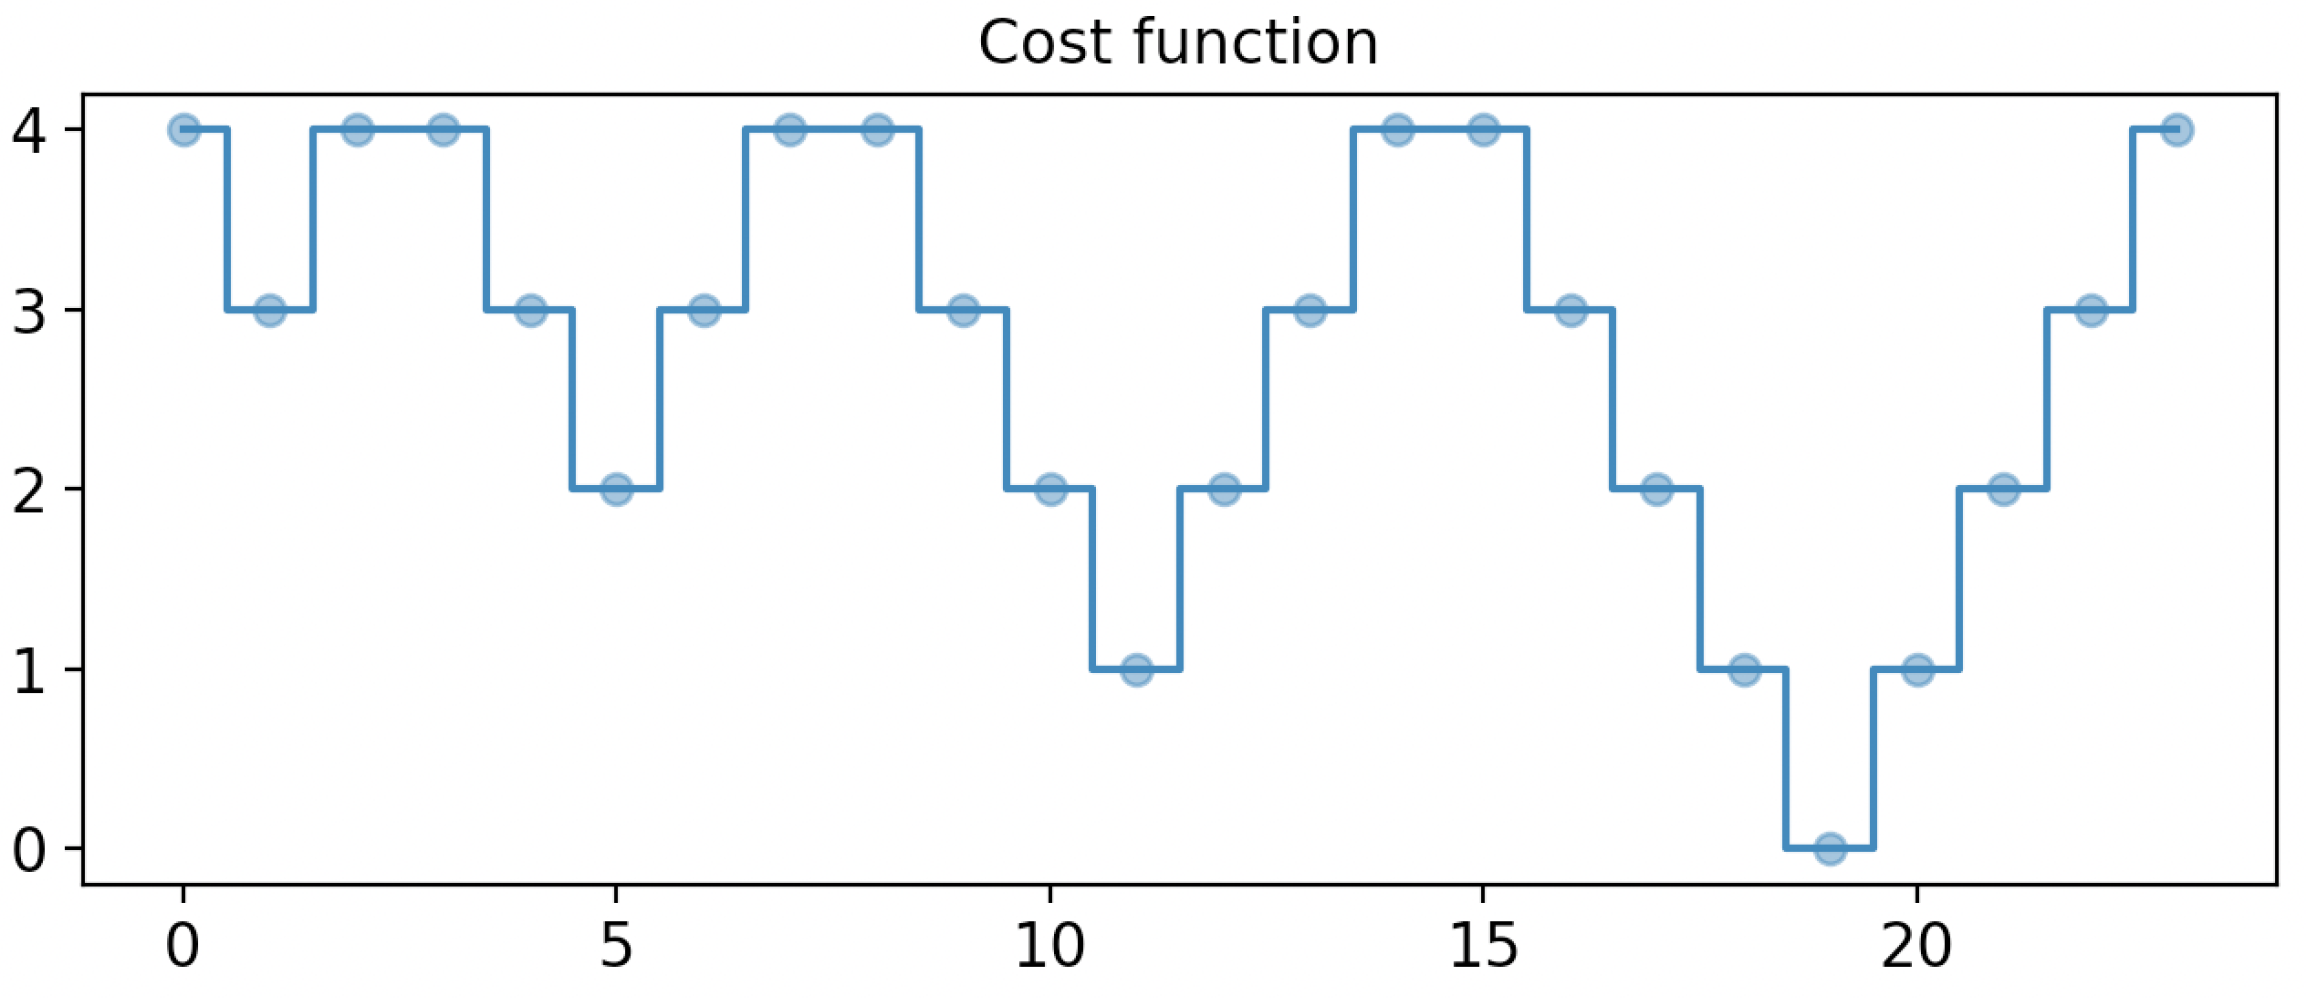
\includegraphics[width=\textwidth]{\dir/chainsaw}
\caption{}
\label{fig:chainsaw_sa}
\end{figure}

Figures~\ref{fig:mcmc_high_temp}--\ref{fig:mcmc_low_temp} depict four Gibbs distributions over $\mathcal{C}$ with different
temperatures. Observe that the higher the temperature, the more uniform
the Gibbs distribution is. In contrast, the lower the temperature, the more
concentrated on $c^*$ the distributions is.

\begin{figure}
    \centering
    \begin{subfigure}[b]{0.6\textwidth}
        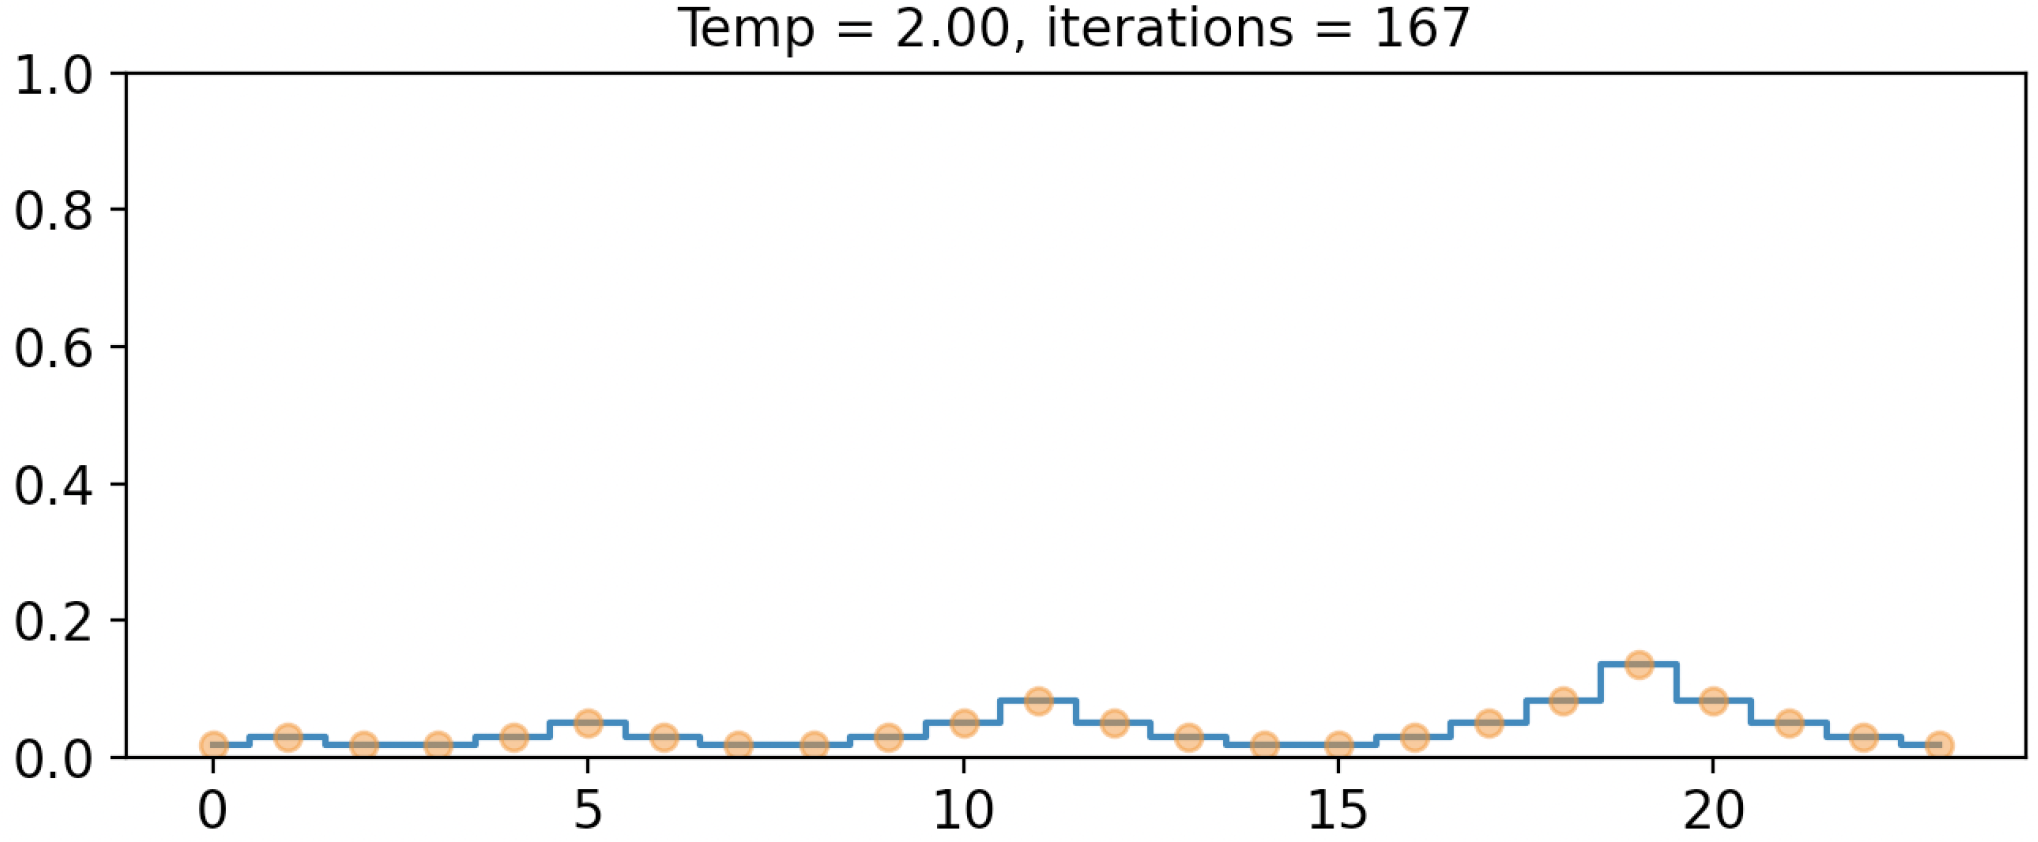
\includegraphics[width=\textwidth]{\dir/mcmc_high_temp}
        \caption{}
        \label{fig:mcmc_high_temp}
    \end{subfigure}

    \begin{subfigure}[b]{0.6\textwidth}
        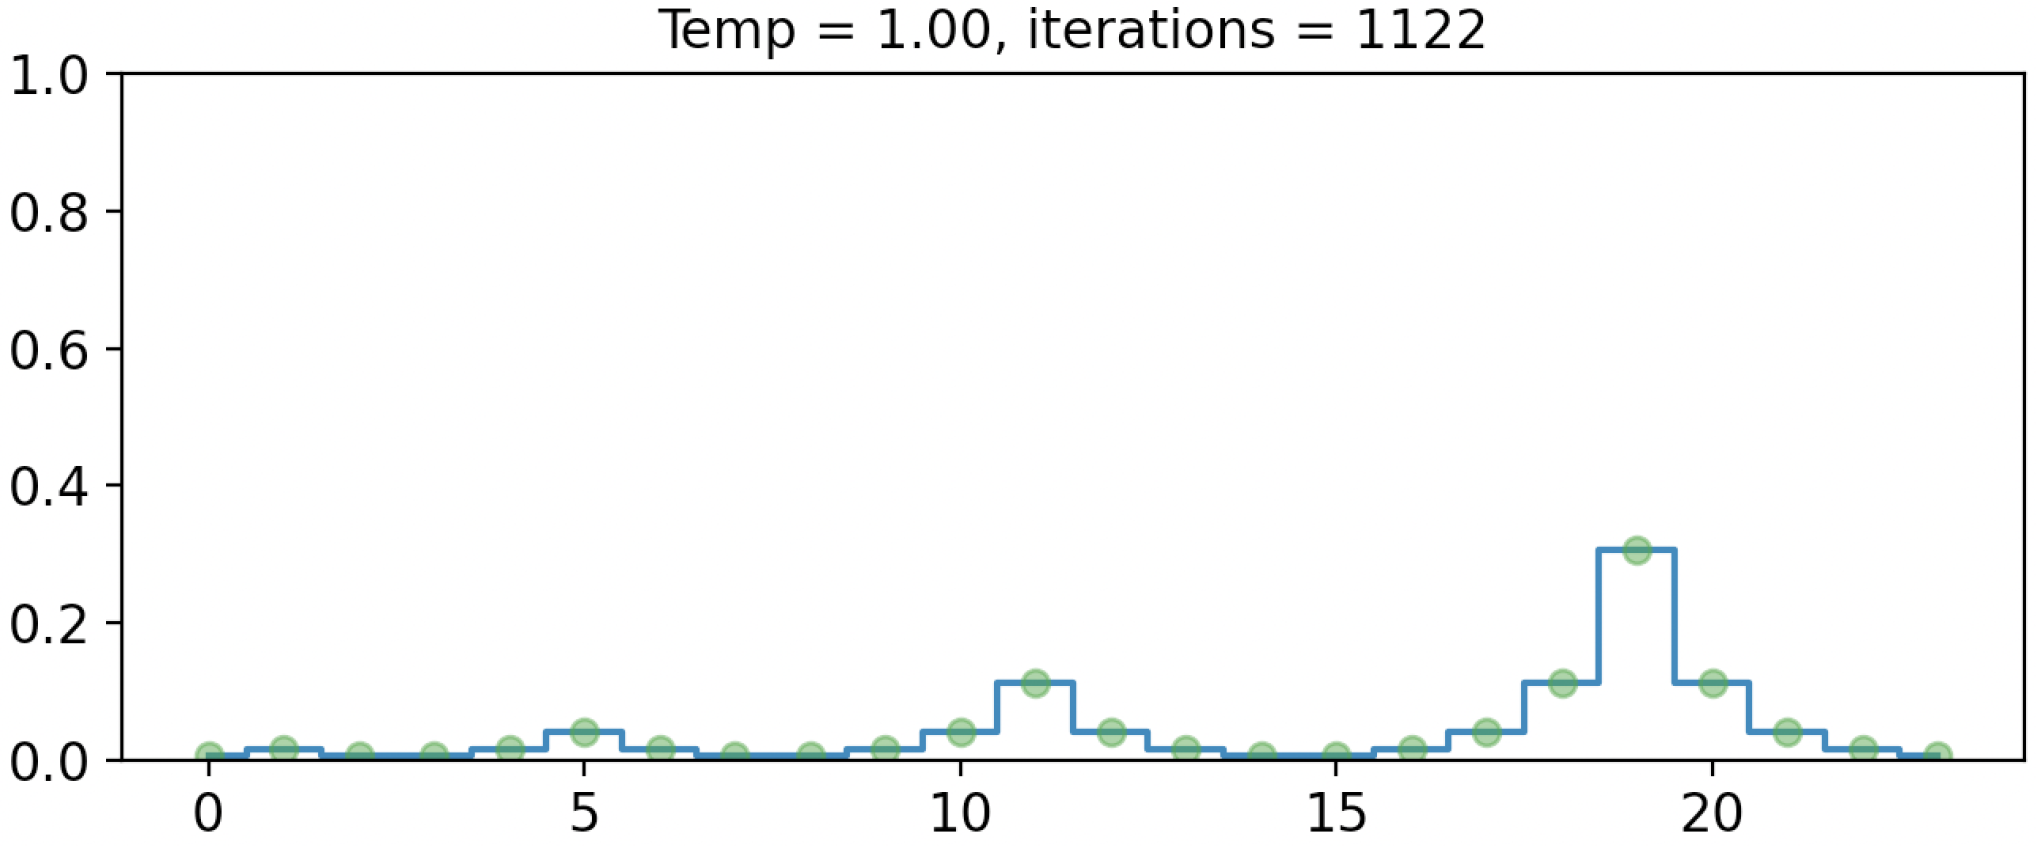
\includegraphics[width=\textwidth]{\dir/mcmc_mid_temp1}
        \caption{}
        \label{fig:mcmc_mid1_temp}
    \end{subfigure}
    
    \begin{subfigure}[b]{0.6\textwidth}
        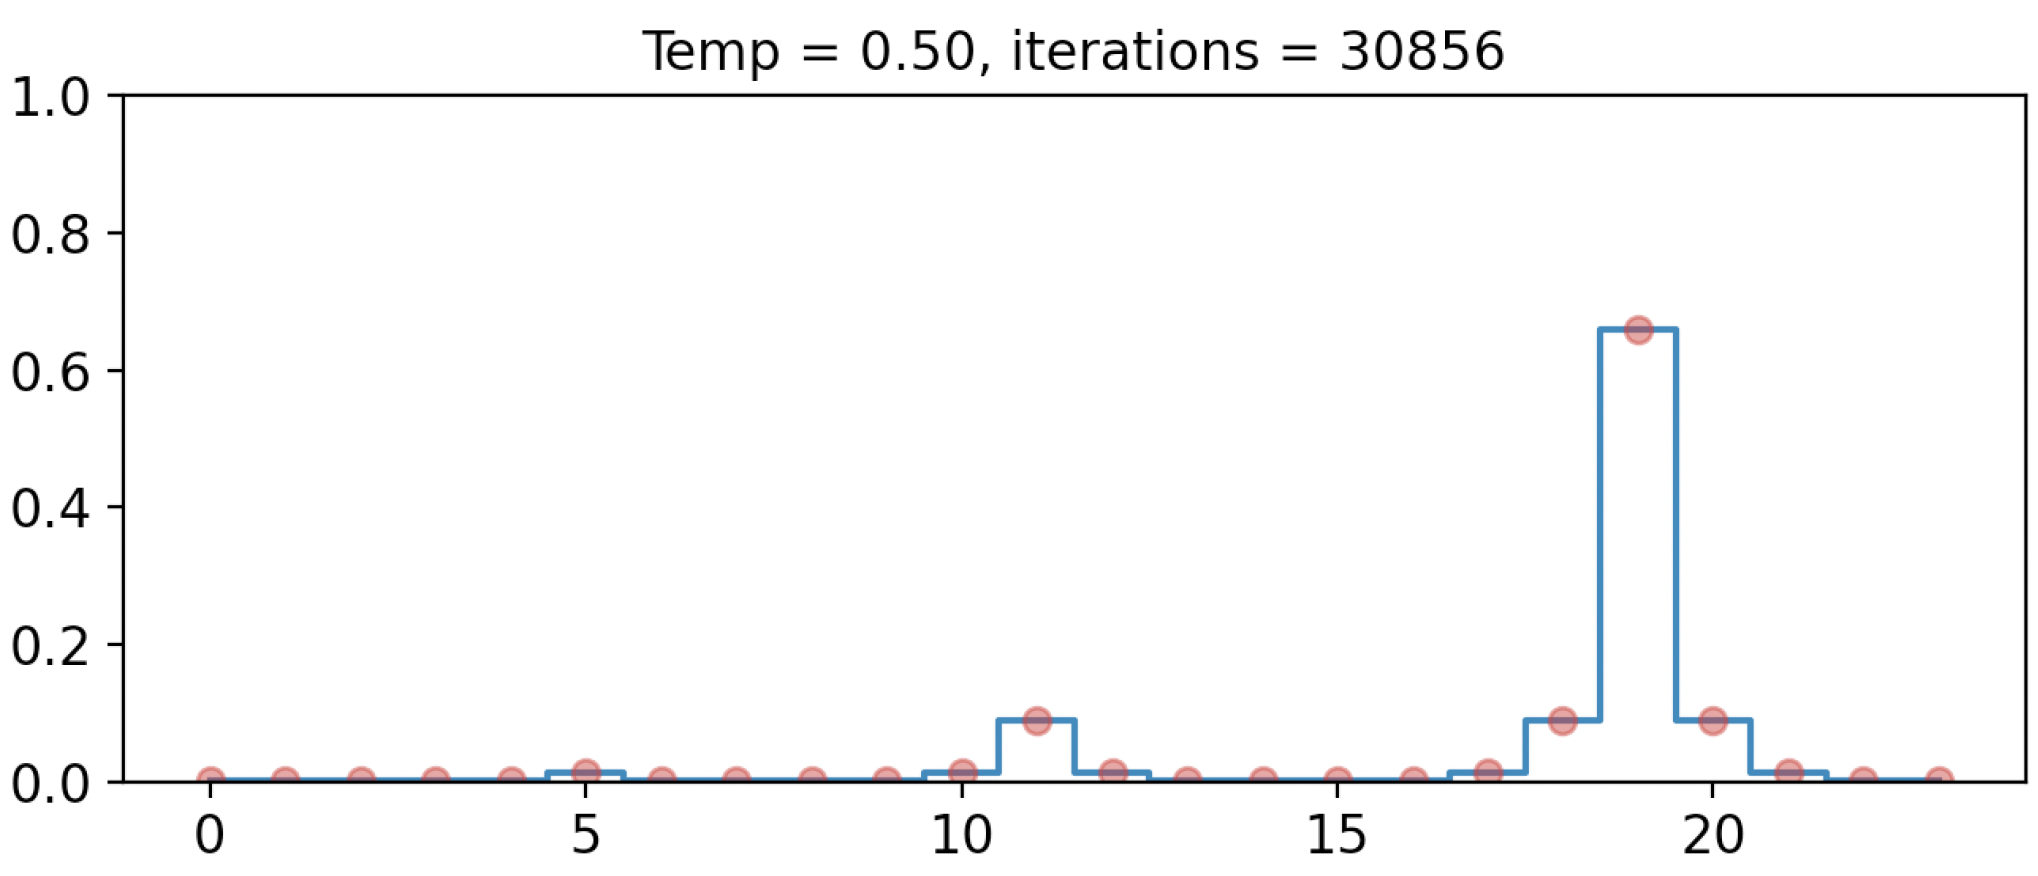
\includegraphics[width=\textwidth]{\dir/mcmc_mid_temp2}
        \caption{}
        \label{fig:mcmc_mid2_temp}
    \end{subfigure}

    \begin{subfigure}[b]{0.6\textwidth}
        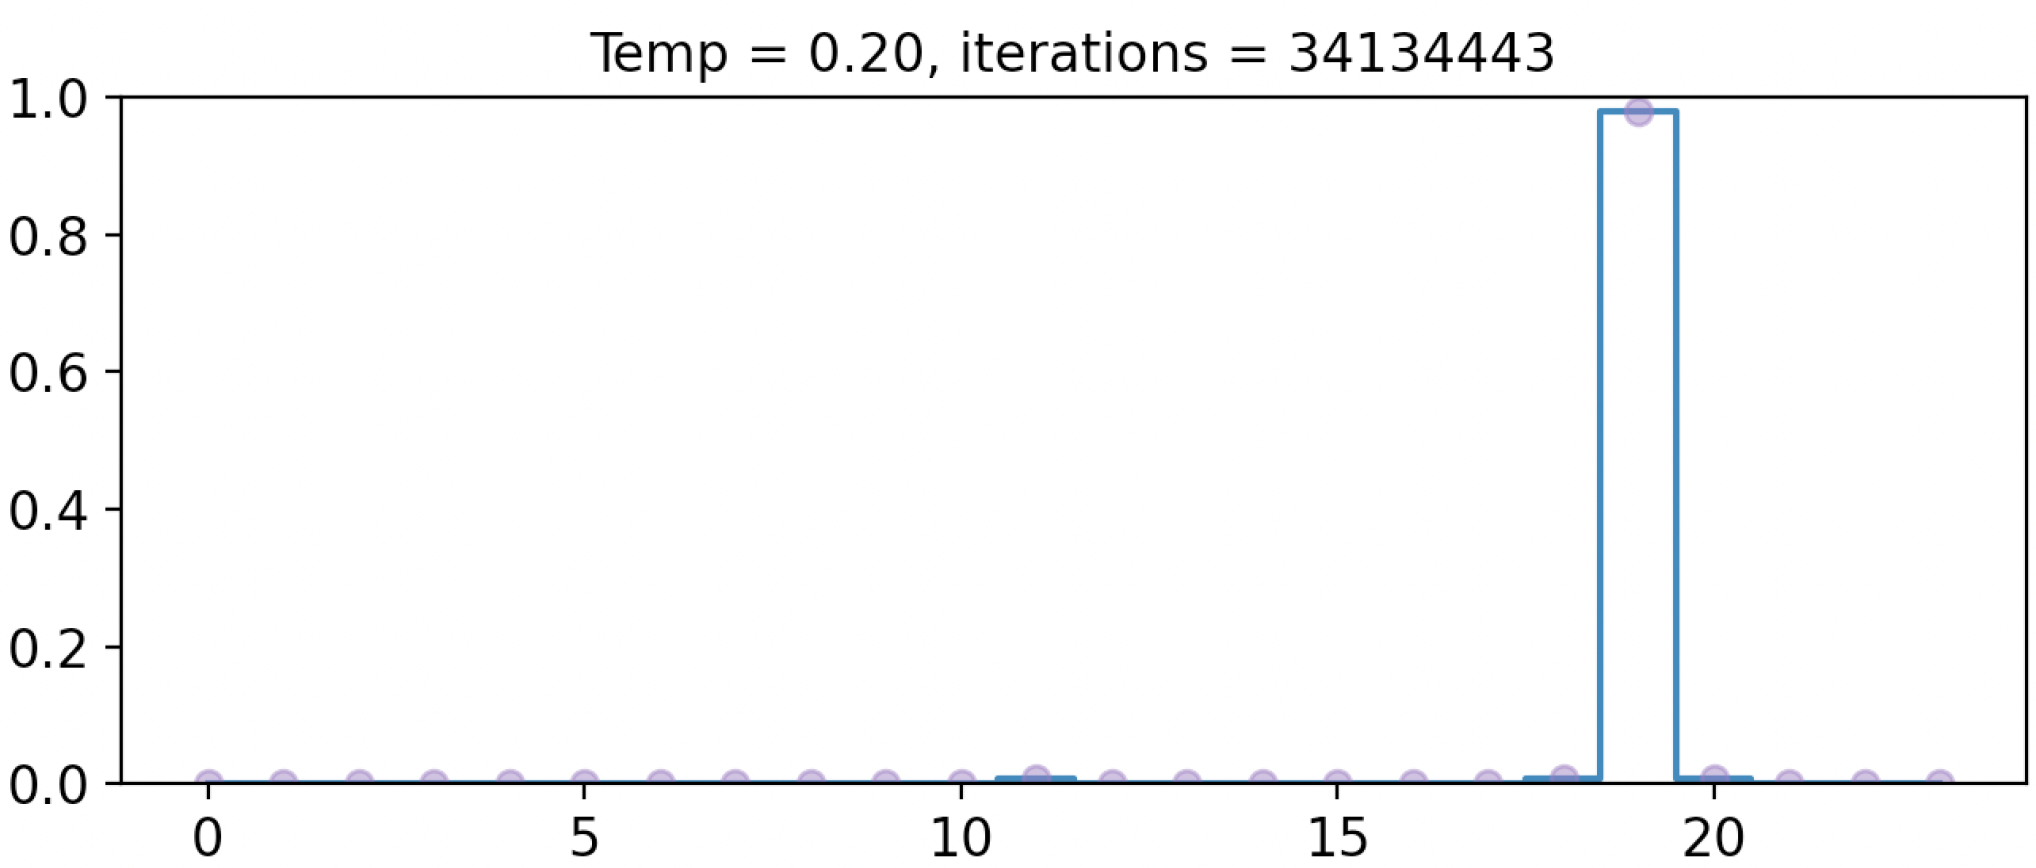
\includegraphics[width=\textwidth]{\dir/mcmc_low_temp}
        \caption{}
        \label{fig:mcmc_low_temp}
    \end{subfigure}
    \caption{Four different Gibbs distributions induced by the cost function
from Figure~\ref{fig:chainsaw_sa}. Observe that the lower the temperature, the more
concentrated the distribution is on the empirical risk minimizer $c^*$. Furthermore,
the number of samples needed to reach $c^*$ from $c_0 = 0$ increases
dramatically as the temperature decreases.}
\end{figure}

\subsection{MCMC as a treasure hunter}

Let us now do MCMC sampling over one of these Gibbs distributions.
We first define a family of proposal $c \in \mathcal{C}$ via
the following randomized algorithm. Assume that you have sampled $c$. To
draw the next sample, flip a coin. If heads comes out, then the next sample
is $c$ again. Otherwise, flip a coin again. If heads comes out, the next sample is $\min(24, c + 1);$ otherwise, it is $\max(0, c - 1)$. More formally,
%
\begin{equation}
q(c' \mid c) =
\begin{cases}
1/4 & \text{if $c' = c + 1$ and $c < 24$},\\
1/4 & \text{if $c' = c + 1$ and $c > 0$},\\
1/2 & \text{if $c' = c$},\\
3/4 & \text{if $c' = c = 0$},\\
3/4 & \text{if $c' = c = 24$}.
\end{cases}
\end{equation}

One can then imagine the MCMC sampling of a Gibbs distribution as a
treasure hunter that randomly traverses the landscape of the cost function
in search for a local minimum of $R(\cdot, X)$. The hunter starts at some location $C_0$. Then it uses the proposal distribution $q(\cdot \mid C_0)$ to choose the location
$C_1$ where it will go next. If $R(C_1, X) \leq R(C_0, X)$, the hunter eagerly
moves to that location. Otherwise, the hunter ponders whether to risk
forgoing the current location, with the hopes that moving to this higher cost
location leads to a location better than the current one. The pondering
is simulated by drawing a sample $B$ from a Bernoulli distribution with
mean $\exp\left(\frac{1}{T}\left(R(C_0, X) - R(C_1, X)\right)\right)$. Observe that the higher $R(C_1, X)$
is with respect to $R(C_0, X)$, the less motivated is the hunter to move to
that location. This motivation is also affected by the temperature. The
lower the temperature, the less motivated is the hunter to move to locations
higher than the current one.

\subsection{The tradeoff induced by the temperature}

Equipped with the intuition of the MCMC sampling algorithm as a treasure
hunter, we report in Figures~\ref{fig:mcmc_high_temp}--\ref{fig:mcmc_low_temp} the number of samples that
we need to draw via MCMC sampling until $c^*$ is sampled for the first time,
when the first sample is $C_0 = 0$. In other words, we report the number
of locations that were visited by the hunter before reaching $c^*$, assuming
that the hunter starts from $C_0 = 0$. Observe that the lower the temperature,
the more samples are needed to draw before sampling $c^*$. This is simply
because in order to reach $c^*$ from $C_0$, the hunter must go through three local
minima before reaching $c^*$. At each local minimum, the hunter must
ponder and choose to forgo the current local minimum. The choice to forgo
becomes more unlikely the more we lower the temperature. This is why
the lower the temperature, the more iterations are needed by the hunter to
reach the $c^*$ for the first time.

The tradeoff induced by the temperature is problematic in practice.
We want a high temperature, so that the hunter is motivated to explore
the landscape of the cost function. However, a high temperature reduces
the ability of the Gibbs distribution to discriminate between good and bad
models because the distribution looks more like a uniform distribution. So
we also want a low temperature, but this negatively affects the hunter's
motivation, making the hunter resistant to leave bad local minima.

\section{Simulated annealing}
\label{sec:simulated_annealing}

Simulated annealing overcomes this tradeoff with a natural solution: start
at a high temperature and then alternate between MCMC sampling and
decreasing the temperature. When the temperature is high, the hunter
roams through the model space. By gradually decreasing the temperature,
we hope that the hunter starts to linger more and more on valuable local
minima. When the temperature becomes significantly low, we hope that
the hunter stays in that local minima. Algorithm~\ref{algo:sa_sa} describes simulated
annealing.

\begin{algorithm}
\begin{algorithmic}[1]
\State Let
\State \quad $\epsilon > 0$ be a temperature threshold.
\State \quad $R(\cdot, X)$ be a cost function,
\State \quad \texttt{reduce} be a function for decreasing the temperature.
\State \quad $q(\cdot \mid c)$, for $c \in \mathcal{C}$, a family of proposal distributions.
\State
\Function{SimAnn}{$\epsilon$, $R(\cdot, X)$, \texttt{reduce}, $\{q(\cdot \mid c) \mid c \in \mathcal{C}\}$}
\State $T \gets \infty$ \Comment{$\infty$ is a sufficiently large value.}
\State $c^T_0 \gets \$$ \Comment{Fix the first element in the sample.}
\While{$T > \epsilon$}
\For{$t = 0\ldots N$}
\State $\tilde{c} \gets \texttt{sample} \; q(\cdot \mid c^T_t)$
\If{$R(\tilde{c}, X) \leq R(c^T_t, X)$}
\State $c^T_{t+1} \gets \tilde{c}$
\Else
\State $b \gets \texttt{sample}$ Bernoulli $\left(\exp\left(\frac{1}{T}\left(R(c^T_t, X)-R(\tilde{c}, X)\right)\right)\right)$
\If{$b = 1$}
\State $c^T_{t+1} \gets \tilde{c}$
\Else
\State $c^T_{t+1} \gets c^T_t$
\EndIf
\EndIf
\EndFor
\State $c_0 \gets c^T_N$ \Comment{Fix the first element for the next sample}
\State $T \gets \texttt{reduce}(T)$
\State $c^T_0 \gets c_0$
\EndWhile
\State \textbf{return} $\left(c^T_t\right)_{T, t}$
\EndFunction
\end{algorithmic}
\caption{Simulated annealing}
\label{algo:sa_sa}
\end{algorithm}

Simulated annealing offers two advantages. First, the gradual temperature
decrease allows the hunter to escape bad local minima, while searching
for the cost function's global minima. So in practice, one can expect that
the cost of simulated annealing's solutions are lower than those from classical
ERM schemes like gradient descent, as they do not have procedures
to escape bad local minima. Second, the sampling nature of simulated annealing
gives us not one but many solutions that are in the ``neighborhood''
of the empirical risk minimizer.

%It is very difficult to diagnose when a Markov chain has burned in.
%Murphy's 24.4.2
